\section{Implementace a publikace}
% Přístup k datům, WMS, WFS, předpřipravené soubory

%\begin{frame}
%\frametitle{Původ dat}
%\begin{center}
%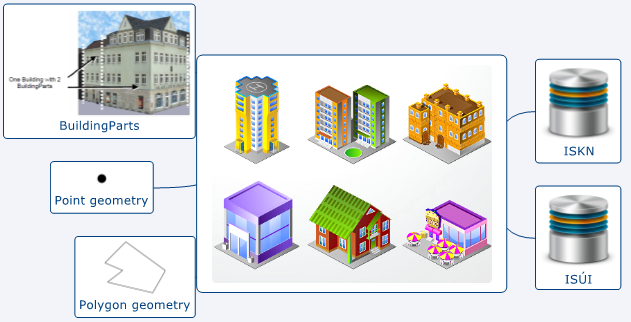
\includegraphics[scale=0.65]{obrazky/various_buildings_possibilities.png}
%\end{center}
%\end{frame}

%\begin{frame}
%\frametitle{Transformace dat}
%\begin{center}
%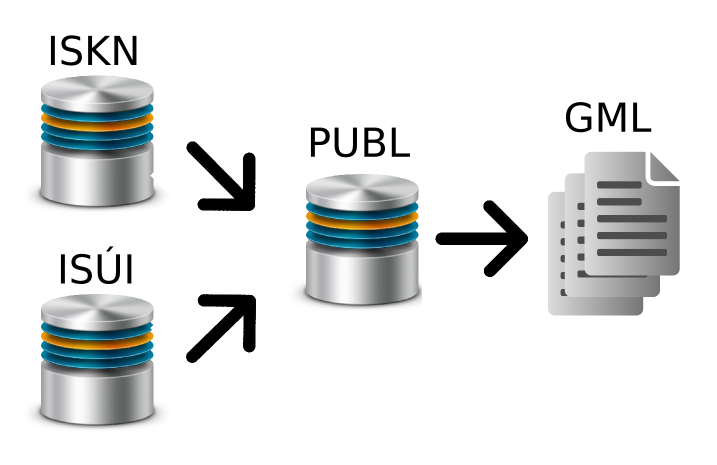
\includegraphics[scale=0.45]{obrazky/transformace.png}
%\end{center}
%\end{frame}

%\begin{frame}
%\frametitle{Publikační databáze -- tabulky}
%\begin{center}
%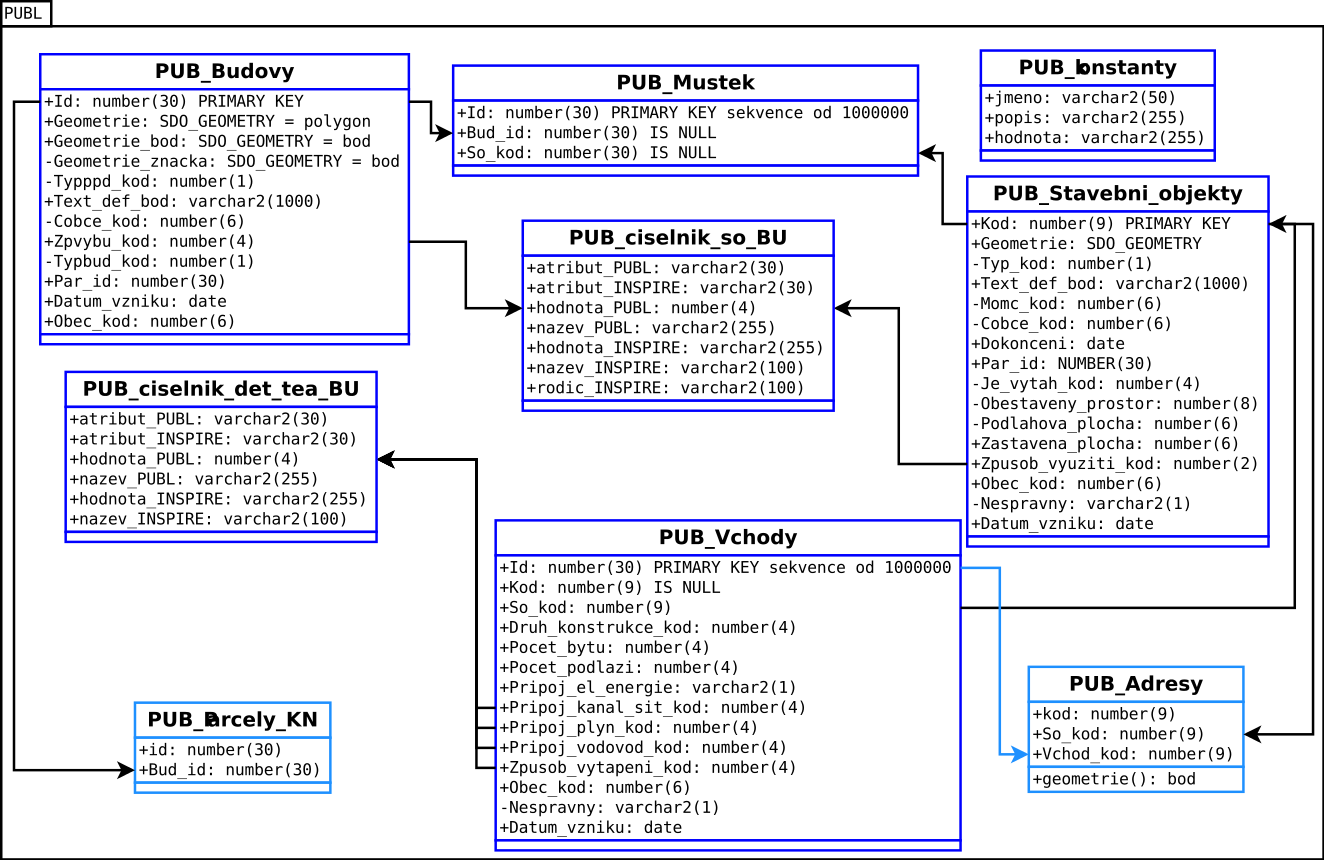
\includegraphics[scale=0.26]{obrazky/BU_PUBL_DB.png}
%\end{center}
%\end{frame}

\begin{frame}
\frametitle{Publikační databáze -- pohledy}
\begin{center}
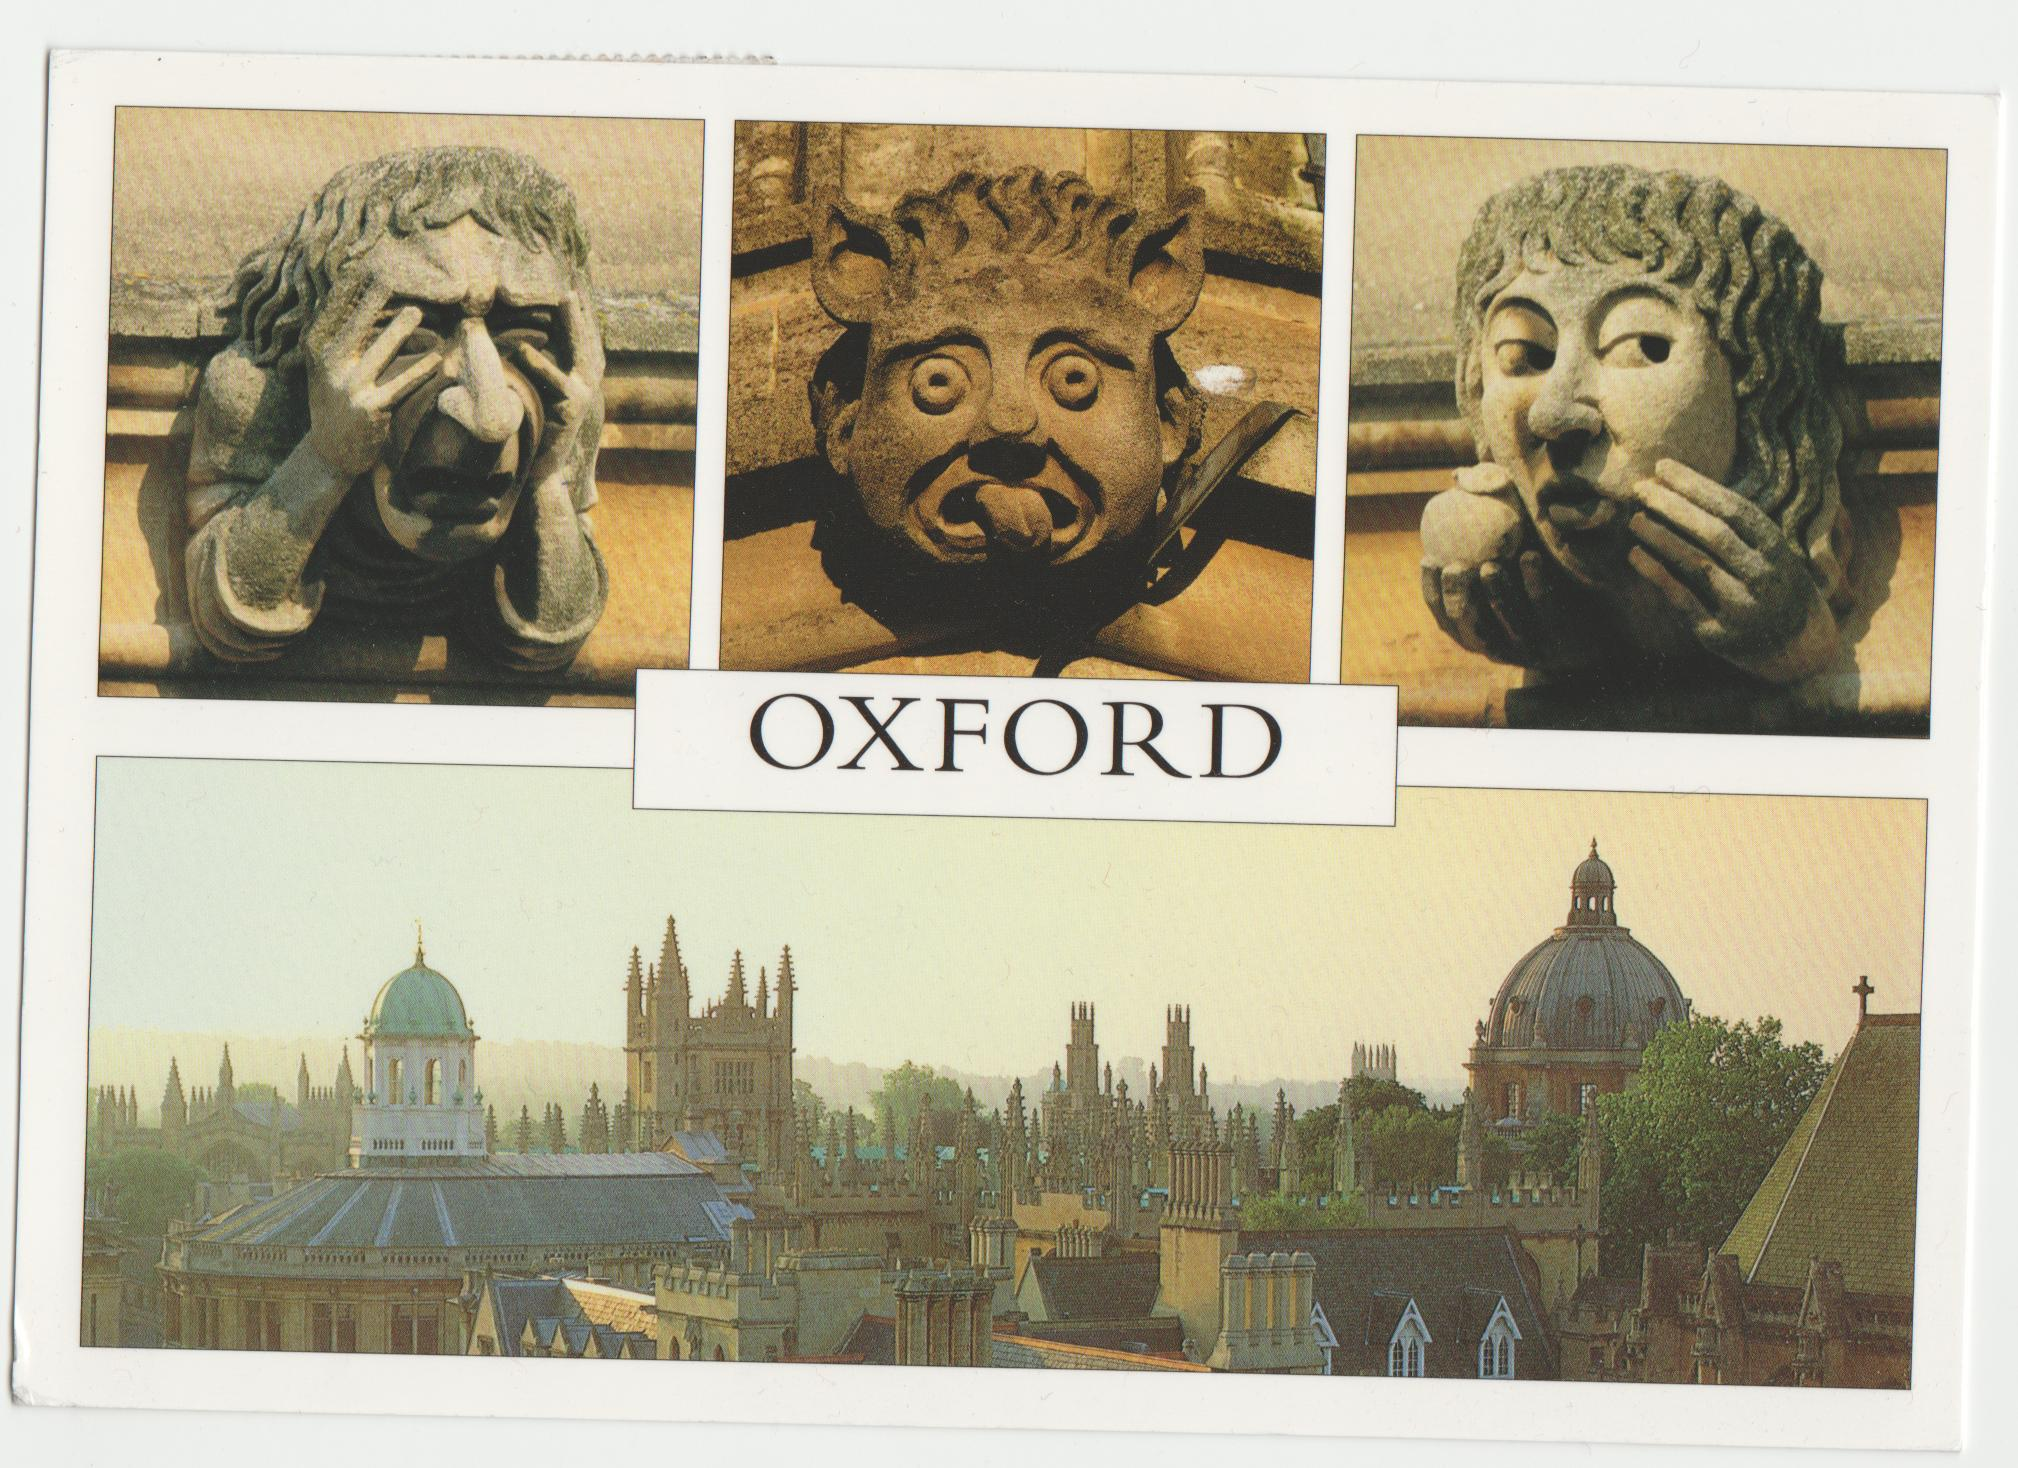
\includegraphics[scale=0.12]{obrazky/pohled.jpg}
\end{center}
\end{frame}

\begin{frame}
\frametitle{Vzorový GML soubor}
\begin{center}
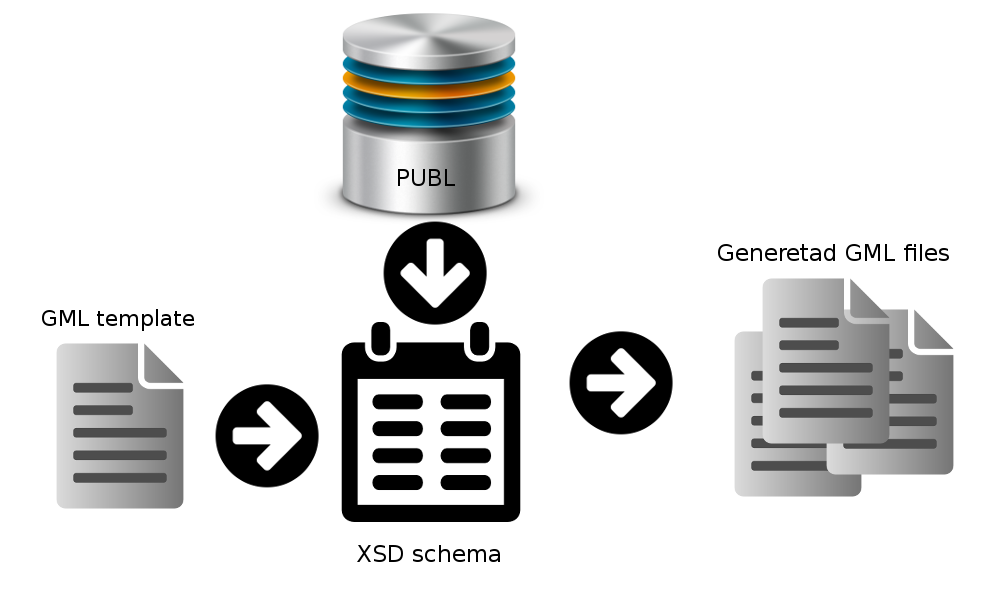
\includegraphics[scale=0.3]{obrazky/GML_sablona.png}
\end{center}
\end{frame}

\begin{frame}
\frametitle{Přístup k datům}
\begin{center}

\includegraphics[scale=0.5]{obrazky/distribuce.png}
\end{center}
\end{frame}

\begin{frame}
\frametitle{Prohlížecí služby -- Building}
\begin{center}
tady bude obrázek wms
\end{center}
\end{frame}

\begin{frame}
\frametitle{Prohlížecí služby -- BuildingPart}
\begin{center}
tady bude obrázek wms
\end{center}
\end{frame}

\begin{frame}
\frametitle{Stahovací služby}
\begin{center}
tady bude obrázek wfs vizualizovaný v QGIS
\end{center}
\end{frame}

\begin{frame}
\frametitle{Předpřipravené GML}
\begin{center}
tady bude obrázek ukazující distribuci pomocí ATOM, WFS nebo vystavením na webu
\end{center}
\end{frame}